\chapter{UI Overview}
\label{sec:ui_overview}

In this section, the main GUI components are described, to give an overview and introduce the different workflow options.

\subfile{ui_main_window}

\section{Main Menu}

\subsection{File Menu}
\label{sec:ui_overview_file_menu}

Databases can be created, opened and closed using the File menu.

\begin{figure}[H]
  \center
    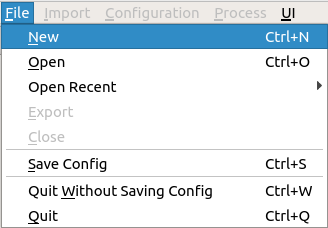
\includegraphics[width=6cm,frame]{figures/ui_file_menu.png}
  \caption{File Menu}
\end{figure}

\begin{itemize}
 \item New: Create new database file
 \item Open: Open existing database file
 \item Open Recent: Open recent existing database file
 \item Export: Create a backup copy of the database file
 \item Close: Close current database
 \item Save Config: Save current configuration
 \item Quit Without Saving Config: Quit application without saving configuration
 \item Quit: Quit application with saving configuration
\end{itemize}
\  \\

After a database was opened, the 'Import' menu becomes available, and the main window looks as follows:

\begin{figure}[H]
  \hspace*{-2.5cm}
    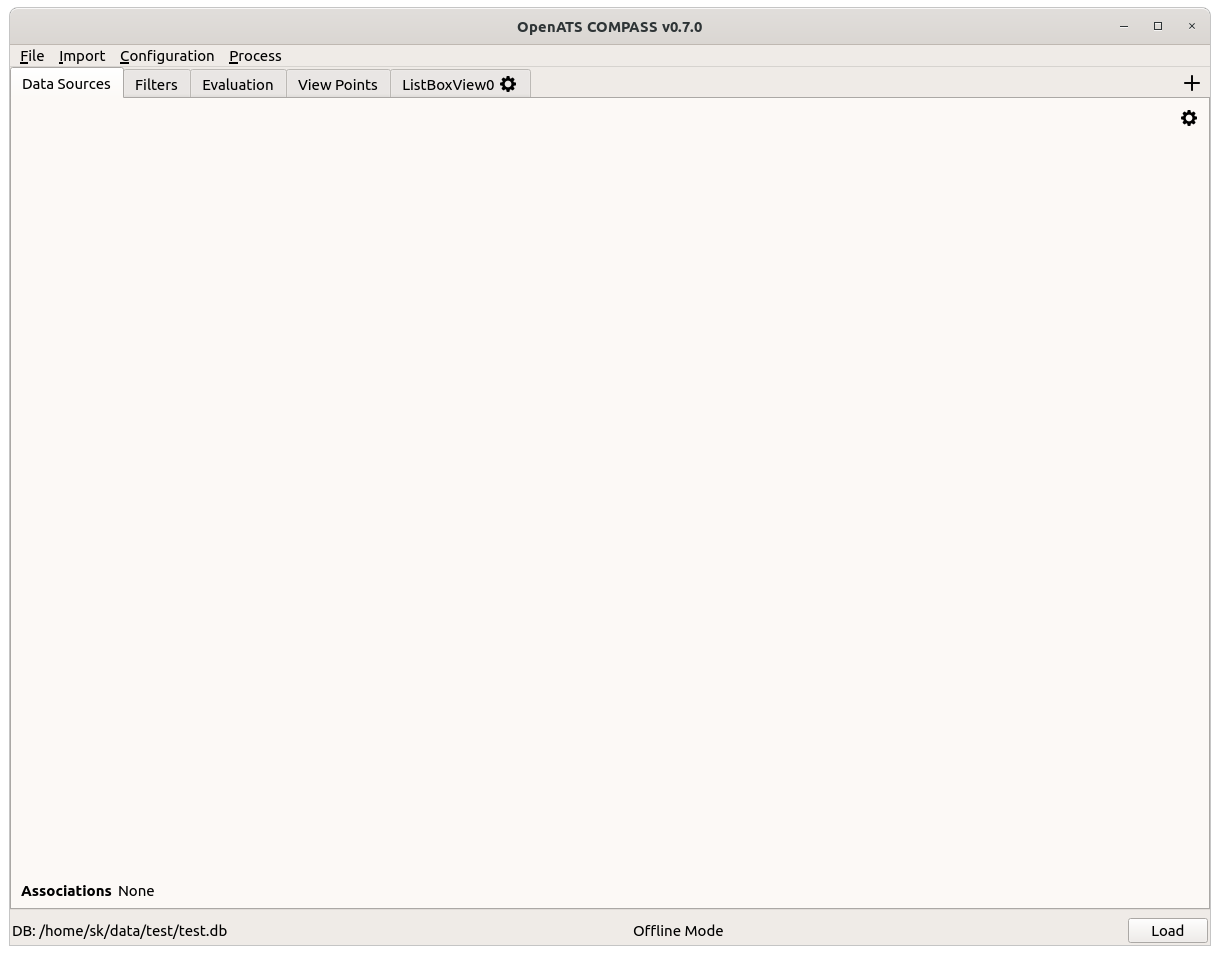
\includegraphics[width=19cm]{figures/main_window_opened.png}
  \caption{Main Window After Opening a Database}
\end{figure}

\subsection{Import Menu}
\label{sec:ui_overview_import_menu}

Data can be imported into the database using the Import menu. This menu is only accessible if a database has been opened.

\begin{figure}[H]
  \center
    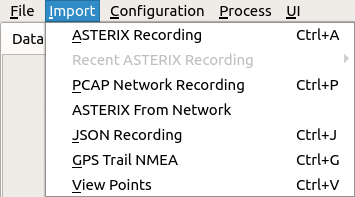
\includegraphics[width=6cm,frame]{figures/ui_import_menu.png}
  \caption{File Menu}
\end{figure}

\begin{itemize}
 \item ASTERIX Recording: Import ASTERIX recording file
 \begin{itemize}
 \item see \nameref{sec:ui_import_asterix}
 \end{itemize}
 \item PCAP Network Recording: Import ASTERIX from a PCAP network recording
  \begin{itemize}
 \item see \nameref{sec:ui_import_pcap}
 \end{itemize}
 \item ASTERIX From Network: Import ASTERIX from network interfaces in Live mode
  \begin{itemize}
 \item see \nameref{sec:ui_import_asterix_network}
 \end{itemize}
 \item JSON Recording: Import JSON recording file
  \begin{itemize}
 \item see \nameref{sec:ui_import_json}
 \end{itemize}
 \item GPS Trail: Import (D)GPS trail from NMEA file
  \begin{itemize}
 \item see \nameref{sec:ui_import_gps}
 \end{itemize}
 \item View Points: Import View Points definition file
  \begin{itemize}
 \item see \nameref{sec:ui_import_viewpoints}
 \end{itemize}
\end{itemize}
\  \\

\subsection{Configuration Menu}
\label{sec:ui_overview_config_menu}

Data sources and sectors can be configured using the Configuration menu. Further, the currently defined Meta Variables can be inspected.

\begin{figure}[H]
  \center
    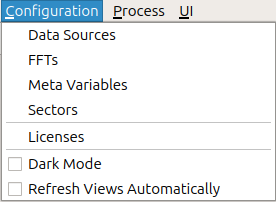
\includegraphics[width=5cm,frame]{figures/ui_configuration_menu.png}
  \caption{Configuration Menu}
\end{figure}

\begin{itemize}
 \item Data Sources: Configure data sources
  \begin{itemize}
 \item see \nameref{sec:ui_configure_data_sources}
 \end{itemize}
 \item Meta Variables: Display current Meta Variables
  \begin{itemize}
 \item see \nameref{sec:configure_meta_vars}
 \end{itemize}
 \item Sectors: Configure sectors in the database
 \begin{itemize}
 \item see \nameref{sec:ui_configure_sectors}
 \end{itemize}
  \item Licenses: Manage licences
 \begin{itemize}
 \item see \nameref{sec:ui_configure_licenses}
 \end{itemize}
\end{itemize}
\  \\

The 'Refresh Views Automatically' checkbox sets if views show trigger an automatic data re-load process if any configuration changes are made (e.g. adding a DBContent variable in TextView, ...).

\subsection{Process Menu}
\label{sec:ui_overview_process_menu}

Post-processing tasks can be performed using the Process menu. This menu is only accessible if a database was opened.

\begin{figure}[H]
  \center
    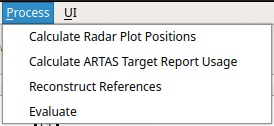
\includegraphics[width=8cm,frame]{figures/ui_process_menu.png}
  \caption{Process Menu}
\end{figure}

\begin{itemize}
 \item Calculate Radar Plot Positions: (Re-)Calculate Radar plot position information
   \begin{itemize}
 \item see \nameref{sec:ui_proc_radar_plot_pos}
 \end{itemize}
 \item Calculate ARTAS Target Report Usage: Associate used target reports to ARTAS tracks based on ARTAS TRI information
   \begin{itemize}
   \item see \nameref{sec:ui_associate_tr_artas}
   \end{itemize}
  \item Reconstruct References: Find unique targets, associate target reports and calculate reference trajectories
   \begin{itemize}
 \item see \nameref{sec:ui_proc_reconst_references}
 \end{itemize}

\end{itemize}
\  \\

\subsection{UI Menu}
\label{sec:ui_overview_ui_menu}

The UI can be reset to a "default" state (as existed at application startup) using the "Reset Views" function.

\subfile{import/ui_import}
\subfile{config/ui_configuration}
\subfile{process/ui_process}
\subfile{ui_ui}
\subfile{ui_data_sources}
\subfile{ui_filters}
\subfile{ui_targets}
\subfile{ui_views}





